
\chapter{Background}
\label{chap:background}

This chapter explains the \textbf{basic concepts} used throughout the thesis. First, we explain \textbf{neural \acp{lm}}: from the basics of neural networks (§\ref{sec:nns}) and language modeling (§\ref{sec:lm-basics}), up to pretrained (§\ref{sec:plms}) and large language models (§\ref{sec:llms}). Then we move on to \textbf{\ac{d2t} generation}: covering rule-based (§\ref{sec:rule-d2t}) and neural-based systems (§\ref{sec:neural-d2t}), \ac{d2t} datasets (§\ref{sec:datasets}) and evaluation methods (§\ref{sec:evaluation}). We assume that the reader has certain expertise in related areas of \ac{nlp}, although not necessarily in \ac{nlg}. We aim to make the work self-contained by covering all the important concepts, pointing the interested reader to related work for more details.

Besides explaining the basic concepts, the chapter serves also as an \textbf{overview of the state of the art} in the field of interest. In particular, the later subsections (\Cref{sec:plms,sec:llms} for neural \acp{lm} and \Cref{sec:neural-d2t,sec:datasets,sec:evaluation} for \ac{d2t} generation) summarize related work and describe the datasets and models used for the experiments. As such, the chapter serves as the main point of reference; we will only briefly revisit the most relevant works in the respective chapters.


\section{Neural Language Models}
\label{sec:lms}
In this section, we work our way towards neural \acp{lm}: the mathematical foundations of \acp{nn} on which the neural \acp{lm} are built on (\autoref{sec:nns}), the basic ideas of language modeling (\autoref{sec:lm-basics}) and the way \acp{lm} are constructed, trained, and eventually applied in \ac{nlp} (\Cref{sec:plms,sec:llms}).

\subsection{Neural Networks}
\label{sec:nns}
First, we need to build a tool for learning patterns from data\footnote{Until we get to \ac{d2t} generation in \autoref{sec:d2t}, we will use the word ``\textit{data}'' only in its abstract sense, as in ``any inputs we can apply our algorithms to''. We will use the term ``structured data'' whenever it is necessary to make the distinction.}. This tool---which for us will be the \textbf{neural networks}---will later help us with learning patterns about language from large-scale textual data, and in turn also with generating the language.

Let's say our goal is to predict the real-number output $y \in \mathbb{R}$ for the given vector of real numbers $\mathbf{x} = (x_1, \ldots, x_n) \in \mathbb{R}^n$.
% \footnote{We will follow the convention that vectors are denoted with boldface letters ($\mathbf{x}$), and real numbers with plain letters ($x$).} 
Let's also assume that the $\mathbf{x} \rightarrow y$ mapping is not arbitrary (that would leave us with memorizing all the $(\mathbf{x},y)$ pairs), but follows some regularities and underlying patterns that can be learned. This assumption will be naturally satisfied if we consider $(\mathbf{x},y)$ to be representations of real-word data, e.g. documents and their labels.

For learning the underlying pattern between $\mathbf{x}$ and $y$, we will use mathematical models designed to capture the pattern in their parameters. The idea is that the models estimate the parameters from a limited set of examples called the \textit{training data}:  $\mathcal{D_{\text{train}}} = \{(\mathbf{x}_1, y_1), \ldots, (\mathbf{x}_{n}, y_{n})\}$, and use the learned parameters to predict the outputs on the \textit{test data}: $\mathcal{D_{\text{test}}} = \{(\mathbf{x}_{n+1}, y_{n+1}), \ldots, (\mathbf{x}_{m}, y_{m})\}$.

\paragraph{Perceptron Algorithm} One of the early mathematical models designed for predicting the outputs based on the inputs is the \emph{perceptron algorithm} \cite{rosenblatt1958perceptron}. In this case, we assume the output is a binary class label: $y \in \{-1, 1\}$. The algorithm learns the parameters $\textbf{w} = (w_1, \ldots, w_n) \in \mathbb{R}^n$ and $b \in \mathbb{R}$ describing a linear decision boundary separating the data points according to their class label. The algorithm proceeds as follows:


\begin{enumerate}
    \item The parameters $\textbf{w}$ and $b$ are initialized to small random values or zeros.
    \item For each training example $(\mathbf{x}_i, y_i)$, the algorithm updates the weights and bias to adjust their current estimate towards the ground truth target:
          \begin{align} \label{eq:perceptron1}
              \hat{y}_i  & = \text{sign}(\textbf{w} \cdot x_i + b)       \\
              \textbf{w} & = \textbf{w} + (y_i - \hat{y}_i) \textbf{x}_i \\
              b          & = b + y_i - \hat{y}_i
          \end{align}
    \item The step (2) is repeated until convergence.
\end{enumerate}

The perceptron algorithm is guaranteed to converge if there exists a hyperplane which separates the data belonging to one class from another. However, it cannot learn a non-linear decision boundary  \cite{novikoff1962convergence}.

\paragraph{Multi-layer Perceptron} To overcome the fact that the perceptron is limited to linear decision boundaries, we can use a \textbf{\ac{mlp}}. This mathematical model---also known as a feed-forward neural network---is able to approximate any bounded continuous function \cite{hornik1989multilayer}.

As the name suggests, \ac{mlp} uses multiple perceptron-like units called \textit{neurons}. Analogically to the perceptron (\autoref{eq:perceptron1}), each neuron computes its output $o$ using the rule:
\begin{align}
    o & = f(\mathbf{w} \cdot \mathbf{x} + b),
\end{align}
% \begin{itemize}
where $f$ is the \emph{activation function}. Instead of signum, \ac{mlp} uses differentiable non-linear functions. The most common activation functions nowadays are \acl{relu} (\acs{relu}; \citealp{nair2010rectified}) or its adapted version \acl{gelu} (\acs{gelu}; \citealp{hendrycks2016gaussian}).

For efficiency, the neurons are organized in layers, which enables formulating the \ac{mlp} computations in terms of matrix multiplication. The $i$-th layer of \ac{mlp} is parametrized with a matrix $\mathbf{W}_i \in \mathbb{R}^{n\times m}$ and a vector of biases $\mathbf{b}_i \in \mathbb{R}^{m}$, performing the following computation:
\begin{align}
    \mathbf{h}_i & = f(\mathbf{W}_i \cdot \mathbf{h}_{i-1} + \mathbf{b}_i).
\end{align}

During training, we aim to minimize the \textit{loss function} describing the gap between the model predictions and the ground truth output. Since all the computations in \ac{mlp} are differentiable, we can use the chain rule to compute how each parameter in the network contributes to the loss. To minimize the loss, we use the \emph{backpropagation} algorithm, updating the network parameters in the reverse order of layers. The magnitude of the updates is controlled by the learning rate parameter $\alpha$.

\paragraph{Recurrent Neural Networks} Unlike \acp{mlp}, where the size of the input $\mathbf{x}$ is fixed, \acp{rnn} allow us to process sequences of arbitrary length. In its vanilla form, the \ac{rnn} maintains a hidden state $\mathbf{h}$ which gets updated for each unit $\mathbf{x}_t$ in sequence using the matrices $\mathbf{W}_h$, $\mathbf{W}_t$, and the bias $\mathbf{b}$.
\begin{align}
    \mathbf{h}_t = f(\mathbf{W}_h \mathbf{h}_{t-1} + \mathbf{W}_x \mathbf{x}_t + \mathbf{b})
\end{align}
\acp{rnn} have various shortcomings, such as repeated updates of the hidden state, which make it difficult to update using gradient-based methods, or inherently sequential processing, making it difficult to paralellize the models. However, they will serve as a springboard towards the Transformer architecture described in \autoref{sec:lm-basics}.


\subsection{Language Modeling}
\label{sec:lm-basics}
We will now look into how can we use neural networks to represent and process text.


\paragraph{One-Hot Encoding} Until now, we have assumed that the input is a vector of real numbers. However, a text is a sequence of discrete units such as characters, words, or subwords. To convert these units---called \textit{tokens}---to a numerical representation, we can define a \textit{vocabulary} $V$ which assigns an integer index $i \in \{0, 1, \ldots, |V|-1\}$ to each token $t$.

The naive way to represent each token would be using its integer value. However, this would misleadingly suggest linear dependence between tokens. A better way is to use the index $i$ for constructing a \textit{one-hot} vector $\mathbf{x} \in \{0,1\}^{|V|} $ for each token:
\begin{align}
    \mathbf{x}[j] = \begin{cases}
        1 & \text{if } i = j, \\
        0 & \text{otherwise}.
    \end{cases}
\end{align}

While this representation is sound, it is sparse and not very helpful for the network. It does not capture the semantics of individual tokens and requires that the network learns to process each token independently.

\paragraph{Word Embeddings} To get a more compact and useful representation of tokens, we may require that the vectors for tokens with a similar role are also close in the vector space. To construct these vectors, we can use the idea that tokens with similar roles also occur in a similar context.

As proposed by \citet{mikolov2013distributed}, we can get these representations as the weights of an \ac{mlp} trained for a particular objective. The \ac{mlp} predicts the tokens in the neighborhood of each token (the \emph{skip-gram} objective) or vice versa, the token itself based on the tokens in its neighborhood (the \textit{continuous bag-of-words} objective), as shown in \autoref{fig:word2vec}.

\begin{figure*}[h]
    \centering

    \begin{subfigure}{\textwidth}
        \centering
        \begin{subfigure}{0.45\textwidth}
            \centering
            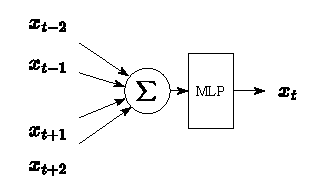
\includegraphics[width=\textwidth]{img/skipgram.pdf}
            \caption{Skip-gram}
            \label{fig:skipgram}
        \end{subfigure}
        \hspace{-20px}
        \begin{subfigure}{0.45\textwidth}
            \centering
            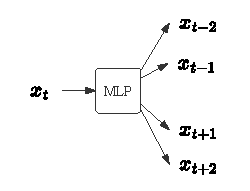
\includegraphics[width=0.75\textwidth]{img/cbow.pdf}
            \caption{Continuous Bag-of-Words}
            \label{fig:cbow}
        \end{subfigure}
    \end{subfigure}
    \caption{The objectives that can be employed by the Word2Vec algorithm for learning token embeddings.}
    \label{fig:word2vec}
\end{figure*}

As a result, we get an \textit{embedding matrix} $\mathbf{W}_e \in \mathbb{R}^{|V|\times d}$, which assigns each token $t \in V$ a $d$-dimensional \textit{embedding vector} $\mathbf{x} \in \mathbb{R}^{d}$.

\paragraph{Tokenization} So far, we have implicitly assumed that we have a way of splitting the text into tokens. Both of the naive approaches---\textit{word-level} and \textit{character-level}---have their own shortcomings. Word-level tokenization will use independent embeddings for morphologically similar words, while character-level tokenization is computationally inefficient.

Subword tokenization algorithms are the middle ground between the two. The goal is to split the text into smaller pieces called \emph{subwords}, so that frequently used words will get their own subword, while less frequent words will be split into multiple subwords.

The algorithm that is frequently used for tokenization in neural \acp{lm} is \textbf{\ac{bpe}}. The \ac{bpe} algorithm starts with the vocabulary of individual bytes, iteratively merging the most frequent tokens and adding them to the vocabulary $V$ until we reach the target vocabulary size. For example, the expression ``Subword tokenization'' could be split into four subwords \texttt{ ['Sub', 'word', '▁token', 'ization']}, the ``\texttt{▁}'' being a special character denoting a preceding space.

\paragraph{Language Modeling} Having a way to represent text, we can move on to processing and subsequently generating it. A useful formalism in that direction is a \textbf{language model}: a mathematical model that estimates a probability $P(T)$ of a sequence of tokens $T = (t_1, \ldots, t_m)$. For estimating the probability, we can factorize it into a product of conditional probabilities for each token using the chain rule:
\begin{align}
    P(T) = \prod_{i=1}^m P(t_i|t_1, \hdots,t_{m-1}).
\end{align}
Estimating the probability of longer sequences according to this formula is infeasible, as the model would require too many parameters. An \textbf{\emph{n}-gram \ac{lm}} simplifies the product using the assumption that the probability of a token depends only on $n-1$ previous tokens:
\begin{align}
    P(T) = \prod_{i=1}^m P(t_i|t_{i-n+1}, \hdots,t_{i-1}).
\end{align}
The \emph{n}-gram \acp{lm} can be trained by estimating probabilities for individual \emph{n}-grams by counting their occurences over a large text corpus. However, because of the simplifying assumption, they fail to capture long-term dependencies in the text.

\paragraph{Neural \acp{lm}} A neural \ac{lm} is a \acl{lm} that estimates the probabilities using a neural network. Denoting the parameters of the network by $\theta$:
\begin{align}
    P(T) = P_\theta(T).
\end{align}
In contrast with \emph{n}-gram \acp{lm}, the neural network can typically process the whole text, efficiently computing the probability estimates using its hidden states. This makes it suitable for capturing long-term dependencies.

A neural network architecture which is suitable for this task is the \ac{rnn} (\autoref{sec:nns}).


\paragraph{Encoder-Decoder Framework}

\paragraph{Transformer Architecture}
% \label{sec:transformer}
\subsection{Pretrained Language Models}
\label{sec:plms}

\paragraph{Encoder Models}

\paragraph{Encoder-Decoder Models}

\paragraph{Decoder Models}

\subsection{Large Language Models}
\label{sec:llms}
\section{Data-to-Text Generation}
\label{sec:d2t}
\subsection{Rule-based Approaches}
\label{sec:rule-d2t}
\subsection{Neural Approaches}
\label{sec:neural-d2t}
\subsection{Datasets}
\label{sec:datasets}
\subsection{Evaluation Metrics}
\label{sec:evaluation}